%%% Template originaly created by Karol Kozioł (mail@karol-koziol.net) and modified for ShareLaTeX use

\documentclass[a4paper,11pt]{article}

\usepackage[T1]{fontenc}
\usepackage[utf8]{inputenc}
\usepackage{graphicx}
\usepackage{subcaption}
\usepackage{xcolor}
\usepackage{stmaryrd}

% \renewcommand\familydefault{\sfdefault}
% \usepackage{tgheros}
% \usepackage[defaultmono]{droidmono}
\usepackage{mathrsfs}

\usepackage{amsmath,amssymb,amsthm,textcomp}
\usepackage{enumerate}
\usepackage{multicol}
\usepackage{tikz}
\usepackage{hyperref}

\usepackage{geometry}
\geometry{left=25mm,right=25mm,%
bindingoffset=0mm, top=20mm,bottom=20mm}

\usepackage[table]{xcolor} % Para colorear tablas
\usepackage{colortbl}      % Necesario para \cellcolor
\usepackage{array}         % Para centrar texto en columnas

\setlength{\parskip}{1em}
%\linespread{1.3}

\newcommand{\linia}{\rule{\linewidth}{0.5pt}}

% % custom theorems if needed
% \newtheoremstyle{mytheor}
%     {1ex}{1ex}{\normalfont}{0pt}{\scshape}{.}{1ex}
%     {{\thmname{#1 }}{\thmnumber{#2}}{\thmnote{ (#3)}}}
%
% \theoremstyle{mytheor}
% \newtheorem{defi}{Definition}

% my own titles
\makeatletter
\renewcommand{\maketitle}{
\begin{center}
\vspace{2ex}
{\Large \textsc{\@title}}
\vspace{1ex}
\\
\linia\\
\@author \hfill \@date
\vspace{4ex}
\end{center}
}
\makeatother
%%%

% custom footers and headers
\usepackage{fancyhdr}
\pagestyle{fancy}
\lhead{}
\chead{}
\rhead{}
%\lfoot{Lógica Proposicional}
\cfoot{}
%\rfoot{página \thepage}
\renewcommand{\headrulewidth}{0pt}
\renewcommand{\footrulewidth}{0pt}
%

% code listing settings
\usepackage{listings}
\lstset{
    language=Python,
    basicstyle=\ttfamily\small,
    aboveskip={1.0\baselineskip},
    belowskip={1.0\baselineskip},
    columns=fixed,
    extendedchars=true,
    breaklines=true,
    tabsize=4,
    prebreak=\raisebox{0ex}[0ex][0ex]{\ensuremath{\hookleftarrow}},
    frame=lines,
    xleftmargin=2em,
    framexleftmargin=2em,
    showtabs=false,
    showspaces=false,
    showstringspaces=false,
    keywordstyle=\color[rgb]{0.627,0.126,0.941},
    commentstyle=\color[rgb]{0.133,0.545,0.133},
    stringstyle=\color[rgb]{01,0,0},
    numbers=left,
    numberstyle=\small,
    stepnumber=1,
    numbersep=5pt,
    captionpos=t,
    escapeinside={\%*}{*)}
}

%% SET THEORY %%

\usepackage{mathtools}
\usepackage{xparse}
\DeclarePairedDelimiterX\set[2]{\{}{\}}{\,#1 \;\delimsize\vert\; #2\,}

\newcommand{\eqdef}{\stackrel{\text{def}}{=}}

%% local labels in equations %%

\usepackage{xargs}

\makeatletter
  \newcommandx{\Label}[1][1={\arabic{equation}}]%
    {\refstepcounter{equation}(\theequation)~\ltx@label{{#1}} &&}
\makeatother

%% Proof trees %%

\usepackage{fitch}

\usepackage{etoolbox}
\let\bbordermatrix\bordermatrix
\patchcmd{\bbordermatrix}{8.75}{4.75}{}{}
\patchcmd{\bbordermatrix}{\left(}{\left[}{}{}
\patchcmd{\bbordermatrix}{\right)}{\right]}{}{}

%% circled question mark %%

\usepackage{tikz}
\newcommand*\circled[1]{\tikz[baseline=(char.base)]{
            \node[shape=circle,draw,inner sep=.7pt] (char) {\footnotesize #1};}}
\newcommand{\result}{\circled{?}}

%% Venn Diagrams %%

\usepackage{venndiagram}

%% LOGICAL SYMBOLS %%

\newcommand{\liff}{\leftrightarrow}
\DeclarePairedDelimiterX\FORALL[3]{(}{)}{\,\forall #1 : #2 : #3 \,}
\DeclarePairedDelimiterX\EXISTS[3]{(}{)}{\,\exists #1 : #2 : #3 \,}
\DeclarePairedDelimiterX\eval[1]{\llbracket}{\rrbracket}{#1}
\newcommand{\sem}[1]{\eval{#1}^{\model}}
\newcommand{\semv}[2]{\eval{#2}^{\model,#1}}
\newcommand{\model}{\mathfrak{M}}
\newcommand{\interpretation}{\mathscr{I}}
\DeclareMathOperator{\dom}{dom}
\DeclareMathOperator{\fun}{fun}
\DeclareMathOperator{\rel}{rel}

\DeclareRobustCommand{\svdots}{% s for `scaling'
  \vcenter{%
    \offinterlineskip
    \vspace{5pt}
    \hbox{.}
    \vskip0.25\normalbaselineskip
    \hbox{.}
    \vskip0.25\normalbaselineskip
    \hbox{.}%
  }%
}

%% COMPLETE BOX %%
\def\fillbox{\quad[\qquad]\quad}

%% NO INDENT %%

\setlength{\parindent}{0pt}

%%%% LOCALDEFS %%%%

\newcommand{\ambassador}{\mathsf{ambassador}_1}
\newcommand{\person}{\mathsf{person}_1}
\newcommand{\country}{\mathsf{country}_1}
\newcommand{\sentto}{\mathsf{sentto}_2}
\newcommand{\knight}{\mathsf{knight}_1}
\newcommand{\knave}{\mathsf{knave}_1}
\newcommand{\alice}{\mathsf{alice}}
\newcommand{\bob}{\mathsf{bob}}
\newcommand{\tom}{\mathsf{tom}}
\newcommand{\carl}{\mathsf{carl}}

\newcommand{\assig}{\cellcolor{gray!30}1}
\newcommand{\conf}{\cellcolor{yellow!40}1}
\newcommand{\void}{\cellcolor{white}0}

%%%----------%%%----------%%%----------%%%----------%%%

\begin{document}

\title{Primer parcial}

\author{Lautaro Luna}

\date{}

\maketitle

\vspace*{-1cm}

\section*{Modelar constelaciones como grafos}
Una constelación es un conjunto de estrellas que, mediante trazos imaginarios, forman un dibujo que
evoca una figura determinada: como un animal, un objeto, o una persona. Estas figuras se basan en
cómo percibimos las posiciones relativas de las estrellas en el cielo, aunque en realidad pueden estar muy
alejadas entre sí en el espacio. Podemos representar una constelación como un grafo, donde cada nodo
es una estrella y cada arista es un trazo imaginario entre dos estrellas. Dado que los trazos que forman
una constelación no tienen una dirección particular, el grafo resultante de la constelación es un grafo no
dirigido, es decir, las aristas se representan como líneas sin dirección


\textbf{Pregunta (a) [2.5 puntos]} \\
Proponga una constelación con al menos 4 (cuatro) aristas. Presente dicha constelación no sólo en
forma gráfica, sino también como un modelo de la lógica (arreglos y matrices). No es necesario que la
constelación propuesta sea una constelación oficialmente aceptada como tal; pueden inventar su propia
constelación, siempre y cuando cumpla con el requisito de cantidad de aristas. \\
Requisitos: Explicar la construcción del modelo y qué representa cada elemento. Elegir una constelación
que tenga un número razonable de estrellas. Usar en la construcción del modelo predicados $star_1$ y
$constellation_2$ los cuales tienen su significado obvio.

\textbf{Pregunta (b) [2.5 puntos]} \\
Describir la constelación propuesta en el punto (a) usando fórmulas. Justificar que el conjunto de fórmulas
describe exactamente la constelación evaluando las fórmulas en el modelo propuesto en el punto (a). \\
Requisitos: Tener en cuenta que las conexiones son sólo entre estrellas, que hay una cantidad precisa
de estrellas en una constelación, y que los trazos en una constelación son unicamente los definidos en la
pregunta (a).

\textbf{Pregunta (c) [2.5 puntos]} \\
Supongamos que tenemos un símbolo de predicado $dreieck_2$ , y símbolos de constante a, b, y c. ¿Qué
tipo de modelos hace verdadero el siguiente conjunto de fórmulas? Justificar la respuesta con un modelo
concreto.

\begin{description}
    \item[(1)] $(a \neq b) \land (b \neq c) \land (a \neq c)$
    \item[(2)] $(\forall s, t :: dreieck_2(s, t) \leftrightarrow (s \neq t) \land ((s = a) \lor (s = b) \lor (s = c)) \land ((t = a) \lor (t = b) \lor (t = c)))$
\end{description}
Requisitos: El modelo debe ser el más chico posible que haga verdaderas las fórmulas (1) y (2).

\textbf{Pregunta (d) [2.5 puntos]} \\
¿Es posible hacer verdaderas las fórmulas (1) y (2) de la pregunta (c) en el modelo de la pregunta (a) si
además agregamos la siguiente fórmula?

\begin{description}
    \item[(3)] $(\forall s, t :: dreieck_2(s, t) \rightarrow constellation_2(s, t))$
\end{description}

Requisitos: Mostrar el resultado de extender el modelo de la pregunta (a) con la interpretación del
símbolo de predicado dreieck2, y los símbolos de constante a, b, y c. Justificar la respuesta evaluando el
conjunto de formulas en el nuevo modelo.

\newpage

\section{Pregunta (a)}

Proponemos el siguiente grafo, compuesto por 10 nodos y 18 aristas. Representa el logo del editor de texto Vim.

\begin{center}
    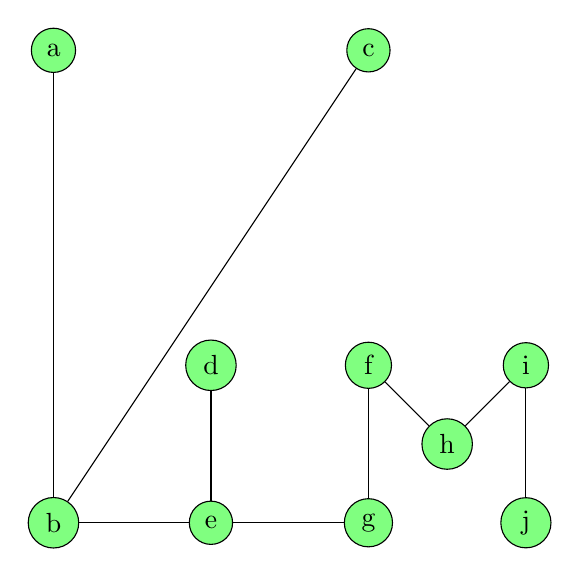
\begin{tikzpicture}
        \node[draw, circle, fill=green!50] (0) at (0,6) {a};
        \node[draw, circle, fill=green!50] (1) at (0,0) {b};
        \node[draw, circle, fill=green!50] (2) at (4,6) {c};
        \node[draw, circle, fill=green!50] (3) at (2,2) {d};
        \node[draw, circle, fill=green!50] (4) at (2,0) {e};
        \node[draw, circle, fill=green!50] (5) at (4,2) {f};
        \node[draw, circle, fill=green!50] (6) at (4,0) {g};
        \node[draw, circle, fill=green!50] (7) at (5,1) {h};
        \node[draw, circle, fill=green!50] (8) at (6,2) {i};
        \node[draw, circle, fill=green!50] (9) at (6,0) {j};

        \draw (0) -- (1);
        \draw (1) -- (2);
        \draw (1) -- (4);
        \draw (3) -- (4);
        \draw (4) -- (6);
        \draw (5) -- (6);
        \draw (5) -- (7);
        \draw (7) -- (8);
        \draw (8) -- (9);
    \end{tikzpicture}
\end{center}

Este grafo se representa a través del siguiente modelo de la lógica.

\begin{center}
    \begin{minipage}{0.1 \textwidth}
        \centering
        \textbf{$\bigtriangleup$} \\[4pt]
        \rowcolors{1}{}{blue!80!white}
        \begin{tabular}{>{\columncolor{blue!80!white}\color{white}\centering}m{1em}}
            0 \\
            1 \\
            2 \\
            3 \\
            4 \\
            5 \\
            6 \\
            7 \\
            8 \\
            9 \\
        \end{tabular}
    \end{minipage}
    \begin{minipage}{0.2 \textwidth}
        \centering
        \textbf{$Constantes$} \\[4pt]
        \begin{tabular}{@{}c@{\hskip 1em}>{\columncolor{blue!80!white}\color{white}}c@{}}
            a & 0 \\
            b & 1 \\
            c & 2 \\
            d & 3 \\
            e & 4 \\
            f & 5 \\
            g & 6 \\
            h & 7 \\
            i & 8 \\
            j & 9 \\
        \end{tabular}
    \end{minipage}
    \begin{minipage}{0.15 \textwidth}
        \centering
        \textbf{$star_1$} \\[4pt]
        \begin{tabular}{@{}c@{\hskip 1em}>{\columncolor{blue!80!white}\color{white}}c@{}}
            0 & 1 \\
            1 & 1 \\
            2 & 1 \\
            3 & 1 \\
            4 & 1 \\
            5 & 1 \\
            6 & 1 \\
            7 & 1 \\
            8 & 1 \\
            9 & 1 \\
        \end{tabular}
    \end{minipage}
    \begin{minipage}{0.4 \textwidth}
        \centering
        \textbf{$constellation_2$} \\[4pt]
        \begin{tabular}{c@{\hskip 1em}*{10}{>{\columncolor{blue!80!white}\color{white}}c}} % Aplica solo a columnas de datos
            % Encabezado (no tiene formato blanco)
            \rowcolor{white}
            \multicolumn{1}{c}{}           &
            \multicolumn{1}{c}{\textbf{0}} &
            \multicolumn{1}{c}{\textbf{1}} &
            \multicolumn{1}{c}{\textbf{2}} &
            \multicolumn{1}{c}{\textbf{3}} &
            \multicolumn{1}{c}{\textbf{4}} &
            \multicolumn{1}{c}{\textbf{5}} &
            \multicolumn{1}{c}{\textbf{6}} &
            \multicolumn{1}{c}{\textbf{7}} &
            \multicolumn{1}{c}{\textbf{8}} &
            \multicolumn{1}{c}{\textbf{9}} &
            \\
            % Cuerpo (tiene fondo azul y texto blanco) 
            0                              & 0 & 1 & 0 & 0 & 0 & 0 & 0 & 0 & 0 & 0 \\
            1                              & 1 & 0 & 1 & 0 & 1 & 0 & 0 & 0 & 0 & 0 \\
            2                              & 0 & 1 & 0 & 0 & 0 & 0 & 0 & 0 & 0 & 0 \\
            3                              & 0 & 0 & 0 & 0 & 1 & 0 & 0 & 0 & 0 & 0 \\
            4                              & 0 & 1 & 0 & 1 & 0 & 0 & 1 & 0 & 0 & 0 \\
            5                              & 0 & 0 & 0 & 0 & 0 & 0 & 1 & 1 & 0 & 0 \\
            6                              & 0 & 0 & 0 & 0 & 1 & 1 & 0 & 0 & 0 & 0 \\
            7                              & 0 & 0 & 0 & 0 & 0 & 1 & 0 & 0 & 1 & 0 \\
            8                              & 0 & 0 & 0 & 0 & 0 & 0 & 0 & 1 & 0 & 1 \\
            9                              & 0 & 0 & 0 & 0 & 0 & 0 & 0 & 0 & 1 & 0 \\
        \end{tabular}
    \end{minipage}
    \begin{minipage}{0.4 \textwidth}
        \centering
        \textbf{$eq_2$} \\[4pt]
        \begin{tabular}{c@{\hskip 1em}*{10}{>{\columncolor{blue!80!white}\color{white}}c}} % Aplica solo a columnas de datos
            % Encabezado (no tiene formato blanco)
            \rowcolor{white}
            \multicolumn{1}{c}{}           &
            \multicolumn{1}{c}{\textbf{0}} &
            \multicolumn{1}{c}{\textbf{1}} &
            \multicolumn{1}{c}{\textbf{2}} &
            \multicolumn{1}{c}{\textbf{3}} &
            \multicolumn{1}{c}{\textbf{4}} &
            \multicolumn{1}{c}{\textbf{5}} &
            \multicolumn{1}{c}{\textbf{6}} &
            \multicolumn{1}{c}{\textbf{7}} &
            \multicolumn{1}{c}{\textbf{8}} &
            \multicolumn{1}{c}{\textbf{9}} &
            \\
            % Cuerpo (tiene fondo azul y texto blanco) 
            0                              & 1 & 0 & 0 & 0 & 0 & 0 & 0 & 0 & 0 & 0 \\
            1                              & 0 & 1 & 0 & 0 & 0 & 0 & 0 & 0 & 0 & 0 \\
            2                              & 0 & 0 & 1 & 0 & 0 & 0 & 0 & 0 & 0 & 0 \\
            3                              & 0 & 0 & 0 & 1 & 0 & 0 & 0 & 0 & 0 & 0 \\
            4                              & 0 & 0 & 0 & 0 & 1 & 0 & 0 & 0 & 0 & 0 \\
            5                              & 0 & 0 & 0 & 0 & 0 & 1 & 0 & 0 & 0 & 0 \\
            6                              & 0 & 0 & 0 & 0 & 0 & 0 & 1 & 0 & 0 & 0 \\
            7                              & 0 & 0 & 0 & 0 & 0 & 0 & 0 & 1 & 0 & 0 \\
            8                              & 0 & 0 & 0 & 0 & 0 & 0 & 0 & 0 & 1 & 0 \\
            9                              & 0 & 0 & 0 & 0 & 0 & 0 & 0 & 0 & 0 & 1 \\
        \end{tabular}
    \end{minipage}
\end{center}

\newpage

Cuenta con un universo $\bigtriangleup$ de 10 elementos, enumerados del 0 al 9. \\
Las constantes para referirse a los nodos son letras de la $a$ a la $j$. Siendo referenciadas de la siguiente manera:\\

\begin{center}
    \begin{tabular}{c c c c c}
        a $\rightarrow$ 0 & b $\rightarrow$ 1 & c $\rightarrow$ 2 & d $\rightarrow$ 3 & e $\rightarrow$ 4 \\
        f $\rightarrow$ 5 & g $\rightarrow$ 6 & h $\rightarrow$ 7 & i $\rightarrow$ 8 & j $\rightarrow$ 9 \\
    \end{tabular}
\end{center}

El arreglo $star_1$ indica si un elemento es una estrella, en este caso, todos los elementos del universo son estrellas.\\
La matriz $constellation_2$ es la matriz de adyacencia, es decir, representa las aristas del grafo. En ella podemos notar que las conexiones entre las estrellas son: \\
\begin{center}
    \begin{tabular}{c c}
        \textbf{a} $\leftrightarrow$ \textbf{b} & \textbf{b} $\leftrightarrow$ \textbf{c} \\
        \textbf{b} $\leftrightarrow$ \textbf{e} & \textbf{d} $\leftrightarrow$ \textbf{e} \\
        \textbf{e} $\leftrightarrow$ \textbf{g} & \textbf{f} $\leftrightarrow$ \textbf{g} \\
        \textbf{f} $\leftrightarrow$ \textbf{h} & \textbf{h} $\leftrightarrow$ \textbf{i} \\
        \textbf{i} $\leftrightarrow$ \textbf{j} &                                         \\
    \end{tabular}
\end{center}

La matriz $eq_2$ representa la relación de igualdad entre elementos del universo. Contiene unos sólo en la diagonal principal, indicando que cada nodo es igual únicamente a sí mismo.

\newpage

\section{Pregunta (b)}

\subsection{Conexiones sólo entre estrellas}
$(\forall s, t :: constellation_2(s, t) \rightarrow (star_1(s) \land star_1(t)))$

\subsection{Hay exactamente 10 estrellas}
$
    (\exists a,b,c,d,e,f,g,h,i,j :: star_1(a) \land star_1(b) \land star_1(c) \land star_1(d) \land star_1(e) \land star_1(f) \land star_1(g) \land star_1(h) \land star_1(i) \land star_1(j))
$

\\
\\

$
    (\exists a,b,c,d,e,f,g,h,i,j ::\;
    a \neq b \land a \neq c \land a \neq d \land a \neq e \land a \neq f \land a \neq g \land a \neq h \land a \neq i \land a \neq j \land{}\\
    b \neq c \land b \neq d \land b \neq e \land b \neq f \land b \neq g \land b \neq h \land b \neq i \land b \neq j \land{}\\
    c \neq d \land c \neq e \land c \neq f \land c \neq g \land c \neq h \land c \neq i \land c \neq j \land{}\\
    d \neq e \land d \neq f \land d \neq g \land d \neq h \land d \neq i \land d \neq j \land{}\\
    e \neq f \land e \neq g \land e \neq h \land e \neq i \land e \neq j \land{}\\
    f \neq g \land f \neq h \land f \neq i \land f \neq j \land{}\\
    g \neq h \land g \neq i \land g \neq j \land{}\\
    h \neq i \land h \neq j \land{}\\
    i \neq j
    )
$

$(\forall x ::\ star_1(x) \Rightarrow (x = a \lor x = b \lor x = c \lor x = d \lor x = e \lor x = f \lor x = g \lor x = h \lor x = i \lor x = j) \big))$


\subsection{Conexiones (aristas) entre estrellas }
$
    (\exists a, b, c, d, e, f, g, h, i, j. :: \\
    constellation_2(a, b) \land constellation_2(b, a) \land \\
    constellation_2(b, c) \land constellation_2(c, b) \land \\
    constellation_2(b, e) \land constellation_2(e, b) \land \\
    constellation_2(d, e) \land constellation_2(e, d) \land \\
    constellation_2(e, g) \land constellation_2(g, e) \land \\
    constellation_2(f, g) \land constellation_2(g, f) \land \\
    constellation_2(f, h) \land constellation_2(h, f) \land \\
    constellation_2(h, i) \land constellation_2(i, h) \land \\
    constellation_2(i, j) \land constellation_2(j, i)
    )
$

\newpage

\subsection{Valuaciones}

\subsubsection{Hay exactamente 10 estrellas}
$
    \begin{nd}
        \hypo{}{(\exists a,b,c,d,e,f,g,h,i,j :: star_1(a) \land star_1(b) \land star_1(c) \land star_1(d) \land star_1(e) \land star_1(f) \land star_1(g) \\
            \land star_1(h) \land star_1(i) \land star_1(j))}
        \have{}{max}
        \open
        \hypo{}{star_1(a) \land star_1(b) \land star_1(c) \land star_1(d) \land star_1(e) \land star_1(f) \land star_1(g) \\
            \land star_1(h) \land star_1(i) \land star_1(j) \\
            cuando [$a = 0, b = 1, c = 2, d = 3, e = 4, f = 5, g = 6, h = 7, i = 8 , j = 9$]}
        \have{}{min(\eval{star_1(a)}, \eval{star_1(b)}, \eval{star_1(c)}, \eval{star_1(d)}, \eval{star_1(e)}, \eval{star_1(f)}, \eval{star_1(g)}, \\
            \eval{star_1(h)}, \eval{star_1(i)}, \eval{star_1(j)},)}
        \open
        \hypo{}{\eval{star_1(a)}}
        \have{}{1}
        \close
        \open
        \hypo{}{\eval{star_1(b)}}
        \have{}{1}
        \close
        \open
        \hypo{}{\eval{star_1(c)}}
        \have{}{1}
        \close
        \open
        \hypo{}{\eval{star_1(d)}}
        \have{}{1}
        \close
        \open
        \hypo{}{\eval{star_1(e)}}
        \have{}{1}
        \close
        \open
        \hypo{}{\eval{star_1(f)}}
        \have{}{1}
        \close
        \open
        \hypo{}{\eval{star_1(g)}}
        \have{}{1}
        \close
        \open
        \hypo{}{\eval{star_1(h)}}
        \have{}{1}
        \close
        \open
        \hypo{}{\eval{star_1(i)}}
        \have{}{1}
        \close
        \open
        \hypo{}{\eval{star_1(j)}}
        \have{}{1}
        \close
        \have{}{1}
        \close
        \have{}{1}
    \end{nd}
$

\newpage



\begin{nd}
    \hypo{}{(\exists a,b,c,d,e,f,g,h,i,j ::\;
        a \neq b \land a \neq c \land a \neq d \land a \neq e \land a \neq f \land a \neq g \land a \neq h \land a \neq i \land a \neq j \land{}\\
        b \neq c \land b \neq d \land b \neq e \land b \neq f \land b \neq g \land b \neq h \land b \neq i \land b \neq j \land{}\\
        c \neq d \land c \neq e \land c \neq f \land c \neq g \land c \neq h \land c \neq i \land c \neq j \land{}\\
        d \neq e \land d \neq f \land d \neq g \land d \neq h \land d \neq i \land d \neq j \land{}\\
        e \neq f \land e \neq g \land e \neq h \land e \neq i \land e \neq j \land{}\\
        f \neq g \land f \neq h \land f \neq i \land f \neq j \land{}\\
        g \neq h \land g \neq i \land g \neq j \land{}\\
        h \neq i \land h \neq j \land{}\\
        i \neq j
        )}
    \have{}{max}
    \open
    \hypo{}{
        a \neq b \land a \neq c \land a \neq d \land a \neq e \land a \neq f \land a \neq g \land a \neq h \land a \neq i \land a \neq j \land{}\\
        b \neq c \land b \neq d \land b \neq e \land b \neq f \land b \neq g \land b \neq h \land b \neq i \land b \neq j \land{}\\
        c \neq d \land c \neq e \land c \neq f \land c \neq g \land c \neq h \land c \neq i \land c \neq j \land{}\\
        d \neq e \land d \neq f \land d \neq g \land d \neq h \land d \neq i \land d \neq j \land{}\\
        e \neq f \land e \neq g \land e \neq h \land e \neq i \land e \neq j \land{}\\
        f \neq g \land f \neq h \land f \neq i \land f \neq j \land{}\\
        g \neq h \land g \neq i \land g \neq j \land{}\\
        h \neq i \land h \neq j \land{}\\
        i \neq j \\
            cuando [$a = 0, b = 1, c = 2, d = 3, e = 4, f = 5, g = 6, h = 7, i = 8 , j = 9$]
    }
    \have{}{min( \eval{a \neq b}, \eval{a \neq c}, \eval{a \neq d}, \eval{a \neq e}, \eval{a \neq f}, \eval{a \neq g}, \eval{a \neq h}, \eval{a \neq i}, \eval{a \neq j},{}\\
        \eval{b \neq c}, \eval{b \neq d}, \eval{b \neq e}, \eval{b \neq f}, \eval{b \neq g}, \eval{b \neq h}, \eval{b \neq i}, \eval{b \neq j},{}\\
        \eval{c \neq d}, \eval{c \neq e}, \eval{c \neq f}, \eval{c \neq g}, \eval{c \neq h}, \eval{c \neq i}, \eval{c \neq j},{}\\
        \eval{d \neq e}, \eval{d \neq f}, \eval{d \neq g}, \eval{d \neq h}, \eval{d \neq i}, \eval{d \neq j},{}\\
        \eval{e \neq f}, \eval{e \neq g}, \eval{e \neq h}, \eval{e \neq i}, \eval{e \neq j},{}\\
        \eval{f \neq g}, \eval{f \neq h}, \eval{f \neq i}, \eval{f \neq j},{}\\
        \eval{g \neq h}, \eval{g \neq i}, \eval{g \neq j},{}\\
        \eval{h \neq i}, \eval{h \neq j},{}\\
        \eval{i \neq j} )}

    \open
    \hypo{}{\eval{a \neq b}}
    \have{}{1}
    \close
    \open
    \hypo{}{\eval{a \neq c}}
    \have{}{1}
    \close
    \open
    \hypo{}{\eval{a \neq d}}
    \have{}{1}
    \close
\end{nd}

\newpage
\begin{nd}
    \open
    \open
    \hypo{}{\eval{a \neq e}}
    \have{}{1}
    \close
    \open
    \hypo{}{\eval{a \neq f}}
    \have{}{1}
    \close
    \open
    \hypo{}{\eval{a \neq g}}
    \have{}{1}
    \close
    \open
    \hypo{}{\eval{a \neq h}}
    \have{}{1}
    \close
    \open
    \hypo{}{\eval{a \neq i}}
    \have{}{1}
    \close
    \open
    \hypo{}{\eval{a \neq j}}
    \have{}{1}
    \close
    \open
    \hypo{}{\eval{b \neq c}}
    \have{}{1}
    \close
    \open
    \hypo{}{\eval{b \neq d}}
    \have{}{1}
    \close
    \open
    \hypo{}{\eval{b \neq e}}
    \have{}{1}
    \close
    \open
    \hypo{}{\eval{b \neq f}}
    \have{}{1}
    \close
    \open
    \hypo{}{\eval{b \neq g}}
    \have{}{1}
    \close
    \open
    \hypo{}{\eval{b \neq h}}
    \have{}{1}
    \close
    \open
    \hypo{}{\eval{b \neq i}}
    \have{}{1}
    \close
    \open
    \hypo{}{\eval{b \neq j}}
    \have{}{1}
    \close
    \open
    \hypo{}{\eval{c \neq d}}
    \have{}{1}
    \close
    \open
    \hypo{}{\eval{c \neq e}}
    \have{}{1}
    \close
    \open
    \hypo{}{\eval{c \neq f}}
    \have{}{1}
    \close
\end{nd}
\newpage
\begin{nd}

    \open
    \open
    \hypo{}{\eval{c \neq g}}
    \have{}{1}
    \close
    \open
    \hypo{}{\eval{c \neq h}}
    \have{}{1}
    \close
    \open
    \hypo{}{\eval{c \neq i}}
    \have{}{1}
    \close
    \open
    \hypo{}{\eval{c \neq j}}
    \have{}{1}
    \close
    \open
    \hypo{}{\eval{d \neq e}}
    \have{}{1}
    \close
    \open
    \hypo{}{\eval{d \neq f}}
    \have{}{1}
    \close
    \open
    \hypo{}{\eval{d \neq g}}
    \have{}{1}
    \close
    \open
    \hypo{}{\eval{d \neq h}}
    \have{}{1}
    \close
    \open
    \hypo{}{\eval{d \neq i}}
    \have{}{1}
    \close
    \open
    \hypo{}{\eval{d \neq j}}
    \have{}{1}
    \close
    \open
    \hypo{}{\eval{e \neq f}}
    \have{}{1}
    \close
    \open
    \hypo{}{\eval{e \neq g}}
    \have{}{1}
    \close
    \open
    \hypo{}{\eval{e \neq h}}
    \have{}{1}
    \close
    \open
    \hypo{}{\eval{e \neq i}}
    \have{}{1}
    \close
    \open
    \hypo{}{\eval{e \neq j}}
    \have{}{1}
    \close
    \open
    \hypo{}{\eval{f \neq g}}
    \have{}{1}
    \close
    \open
    \hypo{}{\eval{f \neq h}}
    \have{}{1}
    \close
    \open
    \hypo{}{\eval{f \neq i}}
    \have{}{1}
    \close
\end{nd}
\newpage
\begin{nd}

    \open
    \open
    \hypo{}{\eval{f \neq j}}
    \have{}{1}
    \close
    \open
    \hypo{}{\eval{g \neq h}}
    \have{}{1}
    \close
    \open
    \hypo{}{\eval{g \neq i}}
    \have{}{1}
    \close
    \open
    \hypo{}{\eval{g \neq j}}
    \have{}{1}
    \close
    \open
    \hypo{}{\eval{h \neq i}}
    \have{}{1}
    \close
    \open
    \hypo{}{\eval{h \neq j}}
    \have{}{1}
    \close
    \open
    \hypo{}{\eval{i \neq j}}
    \have{}{1}
    \close
    \have{}{1}
    \close
    \have{}{1}
\end{nd}

\newpage

\newpage
\begin{nd}
    \hypo{}{(\forall x ::\ star_1(x) \Rightarrow (x = a \lor x = b \lor x = c \lor x = d \lor x = e \lor x = f \lor x = g \lor x = h \lor x = i \lor x = j)}
    \have{}{min}
    \open
    \hypo{}{\eval{star_1(x) \Rightarrow (x = a \lor x = b \lor x = c \lor x = d \lor x = e \lor x = f \lor x = g \lor x = h \lor x = i \lor x = j)} \\ \textbf{ cuando [$x \in [0,9]$]}}
    \have{}{max(1 - \eval{star_1(x)}, (x = a \lor x = b \lor x = c \lor x = d \lor x = e \lor x = f \lor x = g \\ \lor x = h \lor x = i \lor x = j))}
    \open
    \hypo{}{\eval{star_1(x)}}
    \have{}{1}
    \close
    \open
    \hypo{}{x = a \lor x = b \lor x = c \lor x = d \lor x = e \lor x = f \lor x = g \lor x = h \lor x = i \lor x = j}
    \have{}{max(\eval{x = a}, \eval{x = b}, \eval{x = c}, \eval{x = d}, \eval{x = e}, \eval{x = f}, \eval{x = g}, \eval{x = h}, \eval{x = i}, \eval{x = j})}

    \have{}{1}
    \close
    \have{}{1}
    \close

    \have{}{1}
\end{nd}

\newpage



\subsubsection{Conexiones (aristas) entre estrellas}
\begin{nd}
    \hypo{}{(\exists a, b, c, d, e, f, g, h, i, j. ::
        (\exists a, b, c, d, e, f, g, h, i, j. :: \\
        constellation_2(a, b) \land constellation_2(b, a) \land constellation_2(b, c) \land \\
        constellation_2(c, b) \land constellation_2(b, e) \land constellation_2(e, b) \land \\
        constellation_2(d, e) \land constellation_2(e, d) \land constellation_2(e, g) \land \\
        constellation_2(g, e) \land constellation_2(f, g) \land constellation_2(g, f) \land \\
        constellation_2(f, h) \land constellation_2(h, f) \land constellation_2(h, i) \land \\
        constellation_2(i, h) \land constellation_2(i, j) \land constellation_2(j, i))
    }
    \have{}{max}
    \open
    \hypo{}{constellation_2(a, b) \land constellation_2(b, a) \land constellation_2(b, c) \land \\
        constellation_2(c, b) \land constellation_2(b, e) \land constellation_2(e, b) \land \\
        constellation_2(d, e) \land constellation_2(e, d) \land constellation_2(e, g) \land \\
        constellation_2(g, e) \land constellation_2(f, g) \land constellation_2(g, f) \land \\
        constellation_2(f, h) \land constellation_2(h, f) \land constellation_2(h, i) \land \\
        constellation_2(i, h) \land constellation_2(i, j) \land constellation_2(j, i))\\
        \texbf{ cuando [$ a = 0, b = 1, c = 2, d = 3, e = 4, f = 5, g = 6, h = 7, i = 8 , j = 9$]}}
    \have{}{min(
        \eval{constellation_2(a, b)}, \eval{constellation_2(b, a)},
        \eval{constellation_2(b, c)}, \eval{constellation_2(c, b)},\\
        \eval{constellation_2(b, e)}, \eval{constellation_2(e, b)},
        \eval{constellation_2(d, e)}, \eval{constellation_2(e, d)},\\
        \eval{constellation_2(e, g)}, \eval{constellation_2(g, e)},
        \eval{constellation_2(f, g)}, \eval{constellation_2(g, f)},\\
        \eval{constellation_2(f, h)}, \eval{constellation_2(h, f)},
        \eval{constellation_2(h, i)}, \eval{constellation_2(i, h)},\\
        \eval{constellation_2(i, j)}, \eval{constellation_2(j, i)}
        )}

    \open
    \hypo{}{\eval{constellation_2(a, b)}}
    \have{}{1}
    \close

    \open
    \hypo{}{\eval{constellation_2(b, a)}}
    \have{}{1}
    \close

    \open
    \hypo{}{\eval{constellation_2(b, c)}}
    \have{}{1}
    \close

    \open
    \hypo{}{\eval{constellation_2(c, b)}}
    \have{}{1}
    \close

    \open
    \hypo{}{\eval{constellation_2(b, e)}}
    \have{}{1}
    \close

    \open
    \hypo{}{\eval{constellation_2(e, b)}}
    \have{}{1}
    \close
\end{nd}
\newpage
\begin{nd}
    \open
    \open
    \hypo{}{\eval{constellation_2(d, e)}}
    \have{}{1}
    \close

    \open
    \hypo{}{\eval{constellation_2(e, d)}}
    \have{}{1}
    \close

    \open
    \hypo{}{\eval{constellation_2(e, g)}}
    \have{}{1}
    \close

    \open
    \hypo{}{\eval{constellation_2(g, e)}}
    \have{}{1}
    \close

    \open
    \hypo{}{\eval{constellation_2(f, g)}}
    \have{}{1}
    \close

    \open
    \hypo{}{\eval{constellation_2(g, f)}}
    \have{}{1}
    \close

    \open
    \hypo{}{\eval{constellation_2(f, h)}}
    \have{}{1}
    \close

    \open
    \hypo{}{\eval{constellation_2(h, f)}}
    \have{}{1}
    \close

    \open
    \hypo{}{\eval{constellation_2(h, i)}}
    \have{}{1}
    \close

    \open
    \hypo{}{\eval{constellation_2(i, h)}}
    \have{}{1}
    \close

    \open
    \hypo{}{\eval{constellation_2(i, j)}}
    \have{}{1}
    \close

    \open
    \hypo{}{\eval{constellation_2(j, i)}}
    \have{}{1}
    \close

    \have{}{1}
    \close

    \have{}{1}
\end{nd}

\newpage
\section{Pregunta (c)}
\subsection{($(a\ne b)\land\ (b\ne c)\land\ (a\ne c)$)}
\subsection{($\forall s, t:: dreieck_2(s, t) \leftrightarrow ( s \neq t \land ( s = a \lor s = b \lor s = c ) \land ( t = a \lor t = b \lor t = c ) )$)}

\begin{center}
    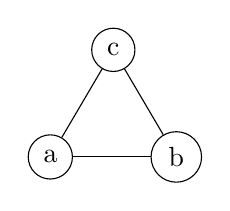
\begin{tikzpicture}[scale=0.8, auto, swap]
        \node (a) at (0,0) [circle, draw ] {a};
        \node (b) at (2,0) [circle, draw ] {b};
        \node (c) at (1,1.7) [circle, draw ] {c};

        \draw (a) -- (b);
        \draw (b) -- (c);
        \draw (c) -- (a);
    \end{tikzpicture}
\end{center}

\begin{center}
    \begin{minipage}{0.2 \textwidth}
        \centering
        \textbf{$Constantes$} \\[4pt]
        \begin{tabular}{@{}c@{\hskip 1em}>{\columncolor{blue!80!white}\color{white}}c@{}}
            a & 0 \\
            b & 1 \\
            c & 2 \\
        \end{tabular}
    \end{minipage}
    \begin{minipage}{0.2\textwidth}
        \centering
        \textbf{$dreieck_2$} \\[4pt]
        \begin{tabular}{c@{\hskip 1em}*{7}{>{\columncolor{blue!80!white}\color{white}}c}}
            % Encabezado con fondo blanco y texto negro
            \rowcolor{white}
            \multicolumn{1}{>{\columncolor{white}\color{black}}c}{}  &
            \multicolumn{1}{>{\columncolor{white}\color{black}}c}{0} &
            \multicolumn{1}{>{\columncolor{white}\color{black}}c}{1} &
            \multicolumn{1}{>{\columncolor{white}\color{black}}c}{2} &

            \\
            % Celdas de la matriz
            0                                                        & 0 & 1 & 1 \\
            1                                                        & 1 & 0 & 1 \\
            2                                                        & 1 & 1 & 0 \\
        \end{tabular}
    \end{minipage}
    \begin{minipage}{0.2\textwidth}
        \centering
        \textbf{$eq_2$} \\[4pt]
        \begin{tabular}{c@{\hskip 1em}*{7}{>{\columncolor{blue!80!white}\color{white}}c}}
            % Encabezado con fondo blanco y texto negro
            \rowcolor{white}
            \multicolumn{1}{>{\columncolor{white}\color{black}}c}{}  &
            \multicolumn{1}{>{\columncolor{white}\color{black}}c}{0} &
            \multicolumn{1}{>{\columncolor{white}\color{black}}c}{1} &
            \multicolumn{1}{>{\columncolor{white}\color{black}}c}{2} &

            \\
            % Celdas de la matriz
            0                                                        & 1 & 0 & 0 \\
            1                                                        & 0 & 1 & 0 \\
            2                                                        & 0 & 0 & 1 \\
        \end{tabular}
    \end{minipage}

\end{center}

\\
\subsection{($(a \neq b)\land\ (b\neq c)\land\ (a\neq c)$)}
\begin{nd}
    \hypo{}{\eval{(a \neq b) \land (b \neq c) \land (a \neq c)}}
    \have{}{\min(\eval{a \neq b},\ \eval{b \neq c},\ \eval{a \neq c})}

    \open
    \hypo{}{\eval{(a \neq b)} }
    \have{}{1}
    \close

    \open
    \hypo{}{\eval{(b \neq c)} }
    \have{}{1}
    \close

    \open
    \hypo{}{\eval{(a \neq c)}}
    \have{}{1}
    \close

    \have{}{1}
\end{nd}

\newpage

\subsection{(\forall s, t:: dreieck_2(s, t) \leftrightarrow ( s \neq t ) \land (( s = a \lor s = b \lor s = c ) \land ( t = a \lor t = b \lor t = c )))}
\begin{nd}
    \hypo{}{\eval{(\forall s, t:: dreieck_2(s, t) \leftrightarrow ( s \neq t ) \land (( s = a \lor s = b \lor s = c ) \land ( t = a \lor t = b \lor t = c )))}}
    \have{}{min}

    \open
    \hypo{}{\eval{dreieck_2(s, t) \leftrightarrow ( s \neq t )\land (( s = a \lor s = b \lor s = c ) \land ( t = a \lor t = b \lor t = c ))} \\
        \textbf{ cuando $[s \in [0,2]$ y $t = s]$}}
    \have{}{1 - |\eval{dreieck_2(s, t)} - \eval{( s \neq t ) \land (( s = a \lor s = b \lor s = c ) \land ( t = a \lor t = b \lor t = c ))} |}

    \open
    \hypo{}{\eval{dreieck_2(s, t)}}
    \have{}{0}
    \close

    \open
    \hypo{}{\eval{( s \neq t )\land (( s = a \lor s = b \lor s = c ) \land ( t = a \lor t = b \lor t = c ))}}
    \have{}{min(\eval{( s \neq t )}, \eval{( s = a \lor s = b \lor s = c ) \land ( t = a \lor t = b \lor t = c )})}

    \open
    \hypo{}{\eval{( s \neq t )}}
    \have{}{0}
    \close



    \have{}{0}

    \close

    \have{}{1}

    \close

\end{nd}
\newpage
\begin{nd}

    \open
    \hypo{}{\eval{dreieck_2(s, t) \leftrightarrow ( s \neq t )\land (( s = a \lor s = b \lor s = c ) \land ( t = a \lor t = b \lor t = c ))} \\
        \textbf{ cuando $[s = 0$ y $t \in [1,2]]$, o bien} \\
        \textbf{ cuando $[s = 1$ y $t \in [0] \cup [2]]$, o bien} \\
        \textbf{ cuando $[s = 2$ y $t \in [0,1]]$, o bien}}
    \have{}{1 - |\eval{dreieck_2(s, t)} - \eval{( s \neq t ) \land (( s = a \lor s = b \lor s = c ) \land ( t = a \lor t = b \lor t = c ))} |}

    \open
    \hypo{}{\eval{dreieck_2(s, t)}}
    \have{}{1}
    \close

    \open
    \hypo{}{\eval{( s \neq t )\land (( s = a \lor s = b \lor s = c ) \land ( t = a \lor t = b \lor t = c ))}}
    \have{}{min(\eval{( s \neq t )}, \eval{( s = a \lor s = b \lor s = c ) \land ( t = a \lor t = b \lor t = c )})}

    \open
    \hypo{}{\eval{( s \neq t )}}
    \have{}{1}
    \close

    \open
    \hypo{}{\eval{( s = a \lor s = b \lor s = c ) \land ( t = a \lor t = b \lor t = c )}}
    \have{}{min(\eval{s = a \lor s = b \lor s = c}, \eval{t = a \lor t = b \lor t = c})}

    \open
    \hypo{}{\eval{s = a \lor s = b \lor s = c}}
    \have{}{max(\eval{s = a}, \eval{s = b}, \eval{s = c})}
    \have{}{1}

    \close

    \open
    \hypo{}{\eval{t = a \lor t = b \lor t = c}}
    \have{}{max(\eval{t = a}, \eval{t = b}, \eval{t = c})}

    \have{}{1}
    \close

    \have{}{1}
    \close

    \have{}{1}

    \close

    \have{}{1}

    \close

    \have{}{1}
\end{nd}


\newpage
\section{Pregunta (d)}
\begin{center}
    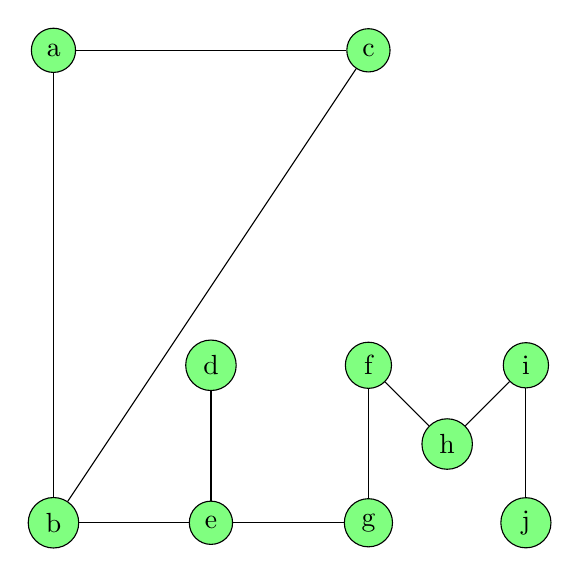
\begin{tikzpicture}
        \node[draw, circle, fill=green!50] (0) at (0,6) {a};
        \node[draw, circle, fill=green!50] (1) at (0,0) {b};
        \node[draw, circle, fill=green!50] (2) at (4,6) {c};
        \node[draw, circle, fill=green!50] (3) at (2,2) {d};
        \node[draw, circle, fill=green!50] (4) at (2,0) {e};
        \node[draw, circle, fill=green!50] (5) at (4,2) {f};
        \node[draw, circle, fill=green!50] (6) at (4,0) {g};
        \node[draw, circle, fill=green!50] (7) at (5,1) {h};
        \node[draw, circle, fill=green!50] (8) at (6,2) {i};
        \node[draw, circle, fill=green!50] (9) at (6,0) {j};

        \draw (0) -- (1);
        \draw (1) -- (2);
        \draw (1) -- (4);
        \draw (3) -- (4);
        \draw (4) -- (6);
        \draw (5) -- (6);
        \draw (5) -- (7);
        \draw (7) -- (8);
        \draw (8) -- (9);
        \draw (0) -- (2);
    \end{tikzpicture}
\end{center}

Este grafo se representa a través del siguiente modelo de la lógica.

\begin{center}
    \begin{minipage}{0.1 \textwidth}
        \centering
        \textbf{$\bigtriangleup$} \\[4pt]
        \rowcolors{1}{}{blue!80!white}
        \begin{tabular}{>{\columncolor{blue!80!white}\color{white}\centering}m{1em}}
            0 \\
            1 \\
            2 \\
            3 \\
            4 \\
            5 \\
            6 \\
            7 \\
            8 \\
            9 \\
        \end{tabular}
    \end{minipage}
    \begin{minipage}{0.2 \textwidth}
        \centering
        \textbf{$Constantes$} \\[4pt]
        \begin{tabular}{@{}c@{\hskip 1em}>{\columncolor{blue!80!white}\color{white}}c@{}}
            a & 0 \\
            b & 1 \\
            c & 2 \\
            d & 3 \\
            e & 4 \\
            f & 5 \\
            g & 6 \\
            h & 7 \\
            i & 8 \\
            j & 9 \\
        \end{tabular}
    \end{minipage}
    \begin{minipage}{0.15 \textwidth}
        \centering
        \textbf{$star_1$} \\[4pt]
        \begin{tabular}{@{}c@{\hskip 1em}>{\columncolor{blue!80!white}\color{white}}c@{}}
            0 & 1 \\
            1 & 1 \\
            2 & 1 \\
            3 & 1 \\
            4 & 1 \\
            5 & 1 \\
            6 & 1 \\
            7 & 1 \\
            8 & 1 \\
            9 & 1 \\
        \end{tabular}
    \end{minipage}
    \begin{minipage}{0.4 \textwidth}
        \centering
        \textbf{$constellation_2$} \\[4pt]
        \begin{tabular}{c@{\hskip 1em}*{10}{>{\columncolor{blue!80!white}\color{white}}c}} % Aplica solo a columnas de datos
            % Encabezado (no tiene formato blanco)
            \rowcolor{white}
            \multicolumn{1}{c}{}           &
            \multicolumn{1}{c}{\textbf{0}} &
            \multicolumn{1}{c}{\textbf{1}} &
            \multicolumn{1}{c}{\textbf{2}} &
            \multicolumn{1}{c}{\textbf{3}} &
            \multicolumn{1}{c}{\textbf{4}} &
            \multicolumn{1}{c}{\textbf{5}} &
            \multicolumn{1}{c}{\textbf{6}} &
            \multicolumn{1}{c}{\textbf{7}} &
            \multicolumn{1}{c}{\textbf{8}} &
            \multicolumn{1}{c}{\textbf{9}} &
            \\
            % Cuerpo (tiene fondo azul y texto blanco) 
            0                              & 0 & 1 & 1 & 0 & 0 & 0 & 0 & 0 & 0 & 0 \\
            1                              & 1 & 0 & 1 & 0 & 1 & 0 & 0 & 0 & 0 & 0 \\
            2                              & 1 & 1 & 0 & 0 & 0 & 0 & 0 & 0 & 0 & 0 \\
            3                              & 0 & 0 & 0 & 0 & 1 & 0 & 0 & 0 & 0 & 0 \\
            4                              & 0 & 1 & 0 & 1 & 0 & 0 & 1 & 0 & 0 & 0 \\
            5                              & 0 & 0 & 0 & 0 & 0 & 0 & 1 & 1 & 0 & 0 \\
            6                              & 0 & 0 & 0 & 0 & 1 & 1 & 0 & 0 & 0 & 0 \\
            7                              & 0 & 0 & 0 & 0 & 0 & 1 & 0 & 0 & 1 & 0 \\
            8                              & 0 & 0 & 0 & 0 & 0 & 0 & 0 & 1 & 0 & 1 \\
            9                              & 0 & 0 & 0 & 0 & 0 & 0 & 0 & 0 & 1 & 0 \\
        \end{tabular}
    \end{minipage}
    \begin{minipage}{0.5 \textwidth}
        \centering
        \textbf{$eq_2$} \\[4pt]
        \begin{tabular}{c@{\hskip 1em}*{10}{>{\columncolor{blue!80!white}\color{white}}c}} % Aplica solo a columnas de datos
            % Encabezado (no tiene formato blanco)
            \rowcolor{white}
            \multicolumn{1}{c}{}           &
            \multicolumn{1}{c}{\textbf{0}} &
            \multicolumn{1}{c}{\textbf{1}} &
            \multicolumn{1}{c}{\textbf{2}} &
            \multicolumn{1}{c}{\textbf{3}} &
            \multicolumn{1}{c}{\textbf{4}} &
            \multicolumn{1}{c}{\textbf{5}} &
            \multicolumn{1}{c}{\textbf{6}} &
            \multicolumn{1}{c}{\textbf{7}} &
            \multicolumn{1}{c}{\textbf{8}} &
            \multicolumn{1}{c}{\textbf{9}} &
            \\
            % Cuerpo (tiene fondo azul y texto blanco) 
            0                              & 1 & 0 & 0 & 0 & 0 & 0 & 0 & 0 & 0 & 0 \\
            1                              & 0 & 1 & 0 & 0 & 0 & 0 & 0 & 0 & 0 & 0 \\
            2                              & 0 & 0 & 1 & 0 & 0 & 0 & 0 & 0 & 0 & 0 \\
            3                              & 0 & 0 & 0 & 1 & 0 & 0 & 0 & 0 & 0 & 0 \\
            4                              & 0 & 0 & 0 & 0 & 1 & 0 & 0 & 0 & 0 & 0 \\
            5                              & 0 & 0 & 0 & 0 & 0 & 1 & 0 & 0 & 0 & 0 \\
            6                              & 0 & 0 & 0 & 0 & 0 & 0 & 1 & 0 & 0 & 0 \\
            7                              & 0 & 0 & 0 & 0 & 0 & 0 & 0 & 1 & 0 & 0 \\
            8                              & 0 & 0 & 0 & 0 & 0 & 0 & 0 & 0 & 1 & 0 \\
            9                              & 0 & 0 & 0 & 0 & 0 & 0 & 0 & 0 & 0 & 1 \\
        \end{tabular}
    \end{minipage}
    \begin{minipage}{0.2\textwidth}
        \centering
        \textbf{$dreieck_2$} \\[4pt]
        \begin{tabular}{c@{\hskip 1em}*{7}{>{\columncolor{blue!80!white}\color{white}}c}}
            % Encabezado con fondo blanco y texto negro
            \rowcolor{white}
            \multicolumn{1}{>{\columncolor{white}\color{black}}c}{}  &
            \multicolumn{1}{>{\columncolor{white}\color{black}}c}{0} &
            \multicolumn{1}{>{\columncolor{white}\color{black}}c}{1} &
            \multicolumn{1}{>{\columncolor{white}\color{black}}c}{2} &

            \\
            % Celdas de la matriz
            0                                                        & 0 & 1 & 1 \\
            1                                                        & 1 & 0 & 1 \\
            2                                                        & 1 & 1 & 0 \\
        \end{tabular}
    \end{minipage}
\end{center}

\newpage
\subsection{Fórmulas}
$(\forall s, t :: dreieck_2(s, t) \rightarrow constellation_2(s, t))$

\begin{nd}
    \hypo{}{\eval{(\forall s, t :: dreieck_2(s, t) \rightarrow constellation_2(s, t))}}
    \have{}{min}
    \open
    \hypo{}{\eval{dreieck_2(s, t) \rightarrow constellation_2(s, t)} \textbf{ cuando $[ s \in [0,2]$ y $t = s$]}}
    \have{}{max(1 - \eval{dreieck_2(s, t)}, \eval{constellation_2(s,t)})}
    \open
    \hypo{}{\eval{dreieck_2(s, t)}}
    \have{}{0}
    \close
    \have{}{1}
    \close

    \open
    \hypo{}{\eval{dreieck_2(s, t) \rightarrow constellation_2(s, t)}
        \textbf{ cuando $[ s = 0$ y $t \in [1,2]$], o bien} \\
        \textbf{ cuando $[ s = 1 $ y $t \in [0] \cup [2]$], o bien} \\
        \textbf{ cuando $[ s = 2 $ y $t \in [0,1]$]} }

    \have{}{max(1 - \eval{dreieck_2(s, t)}, \eval{constellation_2(s,t)})}
    \open
    \hypo{}{\eval{dreieck_2(s, t)}}
    \have{}{1}
    \close
    \open
    \hypo{}{\eval{constellation_2(s, t)}}
    \have{}{1}
    \close
    \have{}{1}
    \close

    \have{}{1}
\end{nd}

\subsection{($(a \neq b)\land\ (b\neq c)\land\ (a\neq c)$)}
\begin{nd}
    \hypo{}{\eval{(a \neq b) \land (b \neq c) \land (a \neq c)}}
    \have{}{\min(\eval{a \neq b},\ \eval{b \neq c},\ \eval{a \neq c})}

    \open
    \hypo{}{\eval{(a \neq b)} }
    \have{}{1}
    \close

    \open
    \hypo{}{\eval{(b \neq c)} }
    \have{}{1}
    \close

    \open
    \hypo{}{\eval{(a \neq c)}}
    \have{}{1}
    \close

    \have{}{1}
\end{nd}

\newpage
\subsection{(\forall s, t:: dreieck_2(s, t) \leftrightarrow ( s \neq t ) \land (( s = a \lor s = b \lor s = c ) \land ( t = a \lor t = b \lor t = c )))}
\begin{nd}
    \hypo{}{\eval{(\forall s, t:: dreieck_2(s, t) \leftrightarrow ( s \neq t ) \land (( s = a \lor s = b \lor s = c ) \land ( t = a \lor t = b \lor t = c )))}}
    \have{}{min}

    \open
    \hypo{}{\eval{dreieck_2(s, t) \leftrightarrow ( s \neq t )\land (( s = a \lor s = b \lor s = c ) \land ( t = a \lor t = b \lor t = c ))} \\
        \textbf{ cuando $[s \in [0,2]$ y $t = s]$}}
    \have{}{1 - |\eval{dreieck_2(s, t)} - \eval{( s \neq t ) \land (( s = a \lor s = b \lor s = c ) \land ( t = a \lor t = b \lor t = c ))} |}

    \open
    \hypo{}{\eval{dreieck_2(s, t)}}
    \have{}{0}
    \close

    \open
    \hypo{}{\eval{( s \neq t )\land (( s = a \lor s = b \lor s = c ) \land ( t = a \lor t = b \lor t = c ))}}
    \have{}{min(\eval{( s \neq t )}, \eval{( s = a \lor s = b \lor s = c ) \land ( t = a \lor t = b \lor t = c )})}

    \open
    \hypo{}{\eval{( s \neq t )}}
    \have{}{0}
    \close



    \have{}{0}

    \close

    \have{}{1}

    \close

\end{nd}
\newpage
\begin{nd}

    \open
    \hypo{}{\eval{dreieck_2(s, t) \leftrightarrow ( s \neq t )\land (( s = a \lor s = b \lor s = c ) \land ( t = a \lor t = b \lor t = c ))} \\
        \textbf{ cuando $[s = 0$ y $t \in [1,2]]$, o bien} \\
        \textbf{ cuando $[s = 1$ y $t \in [0] \cup [2]]$, o bien} \\
        \textbf{ cuando $[s = 2$ y $t \in [0,1]]$, o bien}}
    \have{}{1 - |\eval{dreieck_2(s, t)} - \eval{( s \neq t ) \land (( s = a \lor s = b \lor s = c ) \land ( t = a \lor t = b \lor t = c ))} |}

    \open
    \hypo{}{\eval{dreieck_2(s, t)}}
    \have{}{1}
    \close

    \open
    \hypo{}{\eval{( s \neq t )\land (( s = a \lor s = b \lor s = c ) \land ( t = a \lor t = b \lor t = c ))}}
    \have{}{min(\eval{( s \neq t )}, \eval{( s = a \lor s = b \lor s = c ) \land ( t = a \lor t = b \lor t = c )})}

    \open
    \hypo{}{\eval{( s \neq t )}}
    \have{}{1}
    \close

    \open
    \hypo{}{\eval{( s = a \lor s = b \lor s = c ) \land ( t = a \lor t = b \lor t = c )}}
    \have{}{min(\eval{s = a \lor s = b \lor s = c}, \eval{t = a \lor t = b \lor t = c})}

    \open
    \hypo{}{\eval{s = a \lor s = b \lor s = c}}
    \have{}{max(\eval{s = a}, \eval{s = b}, \eval{s = c})}
    \have{}{1}

    \close

    \open
    \hypo{}{\eval{t = a \lor t = b \lor t = c}}
    \have{}{max(\eval{t = a}, \eval{t = b}, \eval{t = c})}

    \have{}{1}
    \close

    \have{}{1}
    \close

    \have{}{1}

    \close

    \have{}{1}

    \close

\end{nd}
\newpage
\begin{nd}

    \open
    \hypo{}{\eval{dreieck_2(s, t) \leftrightarrow ( s \neq t )\land (( s = a \lor s = b \lor s = c ) \land ( t = a \lor t = b \lor t = c ))} \\
        \textbf{ cuando $[s \in [0,2]$ y $t \in [3,9]]$}}
    \have{}{1 - |\eval{dreieck_2(s, t)} - \eval{( s \neq t ) \land (( s = a \lor s = b \lor s = c ) \land ( t = a \lor t = b \lor t = c ))} |}

    \open
    \hypo{}{\eval{dreieck_2(s, t)}}
    \have{}{0}
    \close

    \open
    \hypo{}{\eval{( s \neq t )\land (( s = a \lor s = b \lor s = c ) \land ( t = a \lor t = b \lor t = c ))}}
    \have{}{min(\eval{( s \neq t )}, \eval{( s = a \lor s = b \lor s = c ) \land ( t = a \lor t = b \lor t = c )})}



    \open
    \hypo{}{\eval{( s = a \lor s = b \lor s = c ) \land ( t = a \lor t = b \lor t = c )}}
    \have{}{min(\eval{s = a \lor s = b \lor s = c}, \eval{t = a \lor t = b \lor t = c})}


    \open
    \hypo{}{\eval{t = a \lor t = b \lor t = c}}
    \have{}{max(\eval{t = a}, \eval{t = b}, \eval{t = c})}

    \have{}{0}
    \close

    \have{}{0}
    \close

    \have{}{0}

    \close

    \have{}{1}

    \close

    \open
    \hypo{}{\eval{dreieck_2(s, t) \leftrightarrow ( s \neq t )\land (( s = a \lor s = b \lor s = c ) \land ( t = a \lor t = b \lor t = c ))} \\
        \textbf{ cuando $[s \in [3,9]$ y $t \in [0,2]]$}}
    \have{}{1 - |\eval{dreieck_2(s, t)} - \eval{( s \neq t ) \land (( s = a \lor s = b \lor s = c ) \land ( t = a \lor t = b \lor t = c ))} |}

    \open
    \hypo{}{\eval{dreieck_2(s, t)}}
    \have{}{0}
    \close

    \open
    \hypo{}{\eval{( s \neq t )\land (( s = a \lor s = b \lor s = c ) \land ( t = a \lor t = b \lor t = c ))}}
    \have{}{min(\eval{( s \neq t )}, \eval{( s = a \lor s = b \lor s = c ) \land ( t = a \lor t = b \lor t = c )})}



    \open
    \hypo{}{\eval{( s = a \lor s = b \lor s = c ) \land ( t = a \lor t = b \lor t = c )}}
    \have{}{min(\eval{s = a \lor s = b \lor s = c}, \eval{t = a \lor t = b \lor t = c})}

    \open
    \hypo{}{\eval{s = a \lor s = b \lor s = c}}
    \have{}{max(\eval{s = a}, \eval{s = b}, \eval{s = c})}
    \have{}{0}

    \close

    \have{}{0}
    \close

    \have{}{0}

    \close

    \have{}{1}

    \close

\end{nd}
\newpage
\begin{nd}

    \open
    \hypo{}{\eval{dreieck_2(s, t) \leftrightarrow ( s \neq t )\land (( s = a \lor s = b \lor s = c ) \land ( t = a \lor t = b \lor t = c ))} \\
        \textbf{ cuando $[s \in [3,9]$ y $t \in [3,9]]$}}
    \have{}{1 - |\eval{dreieck_2(s, t)} - \eval{( s \neq t ) \land (( s = a \lor s = b \lor s = c ) \land ( t = a \lor t = b \lor t = c ))} |}

    \open
    \hypo{}{\eval{dreieck_2(s, t)}}
    \have{}{0}
    \close

    \open
    \hypo{}{\eval{( s \neq t )\land (( s = a \lor s = b \lor s = c ) \land ( t = a \lor t = b \lor t = c ))}}
    \have{}{min(\eval{( s \neq t )}, \eval{( s = a \lor s = b \lor s = c ) \land ( t = a \lor t = b \lor t = c )})}



    \open
    \hypo{}{\eval{( s = a \lor s = b \lor s = c ) \land ( t = a \lor t = b \lor t = c )}}
    \have{}{min(\eval{s = a \lor s = b \lor s = c}, \eval{t = a \lor t = b \lor t = c})}

    \open
    \hypo{}{\eval{s = a \lor s = b \lor s = c}}
    \have{}{max(\eval{s = a}, \eval{s = b}, \eval{s = c})}
    \have{}{0}

    \close

    \have{}{0}
    \close

    \have{}{0}

    \close

    \have{}{1}

    \close

    \have{}{1}
\end{nd}


\end{document}
